\section{Boundary layer}
To introduce the concept of a boundary layer, one has to think of a uniform flow
in one direction with a certain speed ($U_{\infty}$). Now place a thin plate
into this flow where its long side aligns with the flow direction. This setup is
know as \textit{flat plate at zero incidence}. At the surface of the wall, the
\textit{no slip condition} must be satisfied. This means, the flow slows down
until it reaches exactly zero at the surface. This slow down does not happen
linearly and a large portion of the flow remains uniform. The flow is slowed
down only near the surface of the plate due to friction forces. This area is
called the \textit{boundary layer} or \textit{frictional layer}. It's thickness
($\delta(x)$) depends on a lot of different factors, but most prominently on its
position from the leading edge. In reality, there is no hard border between the
uniform flow and the boundary layer. Thus it is often defined as where the flow
reaches 99\% of the velocity of the outer flow \cite{Schlichting2018}. Figure
\ref{fig:boundary_layer_flat_plate} shows this concept.

\begin{figure}[H] \centering
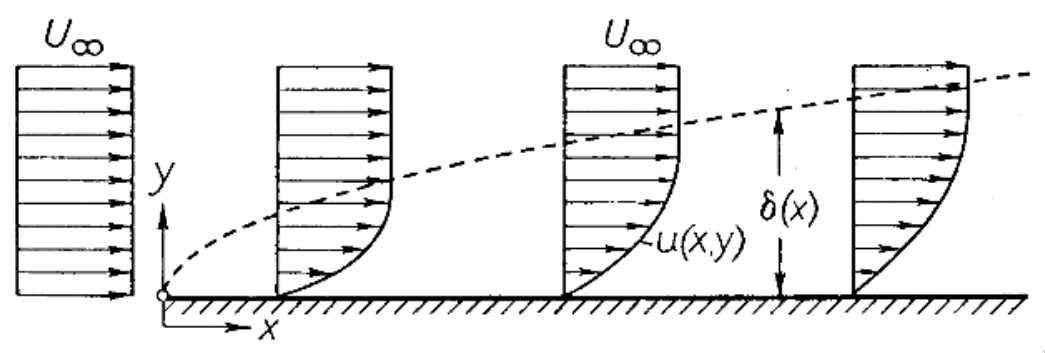
\includegraphics[width=0.5\textwidth]{boundary_layer_flat_plate}
    \caption{Laminar boundary layer of a flat plate at zero incidence \cite{Schlichting2018}.}
    \label{fig:boundary_layer_flat_plate}
\end{figure}

\paragraph{Types of boundary layers}
The flow inside the boundary layer might be \textit{laminar} or
\textit{turbulent}. In reality, it is laminar at the leading edge, transitions
to turbulence over a certain length and becomes fully turbulent afterwards
\cite{Schlichting2018}. As this report deals with a fully turbulent
\textit{turbulence model}, the first two types of boundary layer are not
explained further.

\paragraph{Frictional forces}
As explained earlier, the flow in the boundary layer is slowed down until it
becomes zero at the surface. This slowing down exerts a force in the flow
direction on the surface. This force, normalized by its application area, is
called \textit{shear stress} ($\tau_{w}$). To obtain a dimensionless
coefficient, which may be easily compared, the shear stress is divided by the
\textit{dynamic pressure} \cite{Schlichting2018}:

\begin{equation}
  c_{f} = \frac{\tau_{w}(x)}{\frac{1}{2}\rho U_{\infty}^{2}}
\end{equation}

\noindent Where $\rho$ is the density of the fluid.


\subsection{Turbulent boundary layer}
When looking closer at a turbulent boundary layer, once can observer two
different regions. At the top is a \textit{turbulent layer} which is only
indirectly affected by the friction with the wall. At the bottom is a layer that
is really thin compared to the boundary layer. It is called \textit{viscous
sublayer} or \textit{viscous wall layer} and is directly affected by the
friction. As is the case with the boundary layer itself, there is no hard border
between those two regions. Instead one can observe a smooth transition
\cite{Schlichting2018}.

To examine the cross section of the boundary layer, it make sens to introduce
the concept of the dimensionless \textit{wall distance} $y^{+}$. Hand in hand
goes the dimensionless velocity $u^{+}$. Moving to this dimensionless system
allows us to compare different boundary layers from different flow conditions
more easily. The velocity $u^{+}$ is given by \cite{jousefm_2020}:

\begin{equation}
  u^{+} = \frac{u}{u_{\tau}}
\end{equation}

\noindent Where as $u$ is the flow velocity and $u_{\tau}$ the \textit{friction velocity}.
It is given by:

\begin{equation}
  u_{\tau} = \sqrt{\frac{\tau_{w}}{\rho}}
\end{equation}

\noindent As before, $\tau_{w}$ is the \textit{shear stress} and $\rho$ the
\textit{density}. The dimensionless \textit{wall distance} $y^{+}$ is given by:

\begin{equation}
  y^{+} = \frac{yu_{\tau}}{\nu}
\end{equation}

\noindent Where as $y$ is the distance to the wall and $\nu$ is the \textit{kinematic
viscosity} of the fluid.


\subsubsection{Law of the wall}
Theory which describes the velocity distribution of a turbulent boundary layer
in fully developed flow\footnote{This means, the flow does not change with
increasing x.}  is know as the \textit{law of the wall}. It defines the
different regions as follows:

\paragraph{Viscous sublayer ($y^{+} < 5$)}
For the viscous sublayer, $u^{+}$ is given by:

\begin{equation}
  u^{+} = y^{+}
\end{equation}

\paragraph{Logarithmic area ($y^{+} > 30$)}
In the fully turbulent region at the top of the boundary layer, the turbulence stress dominates and the velocity profile varies very slowly with a logarithmic function:

\begin{equation}
  u^{+} = \frac{1}{\kappa} ln(y^{+}) + B
\end{equation}

\noindent The Karman constant $\kappa$ is equal to $0.41$ and $B$ equals to $5.2$.

\paragraph{Buffer layer ($5 < y^{+} < 30$)}
The \textit{buffer layer} is located between the viscous sublayer and the
logarithmic area. It is a region where the flow transitions from one to the
other and is not well defined.

If we plot the wall distance $y^{+}$ on a logarithmic scale and the velocity
$u^{+}$ on a linear scale, the different regions are obvious. Take a look at
figure \ref{fig:law_of_wall}.

\begin{figure}[H] \centering
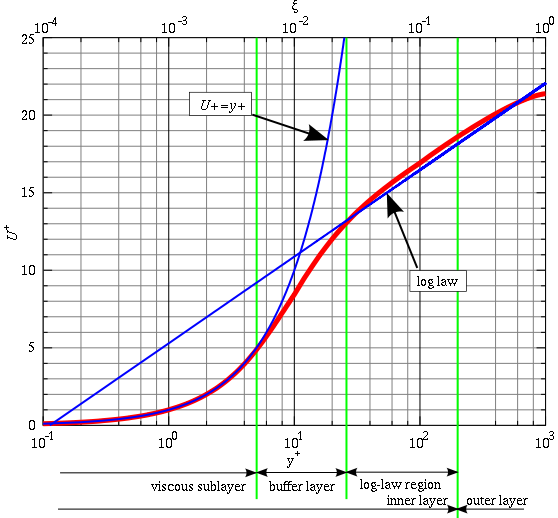
\includegraphics[width=0.7\textwidth]{law_of_wall}
    \caption{Cross section of a fully developed turbulent boundary layer \cite{jousefm_2020}.}
    \label{fig:law_of_wall}
\end{figure}





\subsection{Turbulent boundary layer over rough walls}



\section{Reynold's Averaged Navier Stokes (RANS)}

\subsection{ADflow}

\subsection{SU2}



\section{Turbulence Models}


\subsection{Spalart Allmaras (SA)}


\subsection{Modification of SA for rough walls}
